\section{Architecture Overview}

The following sections describe the framework that builds the foundations to design rapport agents using a plugin-based paradigm that takes into account the current limitations of the \ac{SERA} framework, and the rapport model detailed in Chapter~\ref{chap:rapportModel}. In order to tackle the delay between the requests and the effect (as described in Section~\ref{sub:sera:features_limitations}), the framework limits the number of network messages by communicating internally though regular method calls and events.

Following Figure~\ref{fig:rapport:archicture}, the framework contains the following elements:
\begin{itemize}
	\item \textbf{\textit{Effector Plugins}}: propose actions and enables/disables plugins;
	\item \textbf{\textit{Perceiver Plugins}}: perceive the external world and informs the interested plugins;
	\item \textbf{\textit{Utility Plugins}}: general purpose plugins that can be used to, for example, store the dyadic state of the interaction;
	\item \textbf{\textit{Rapport Controller}}: manages plugins' lifecycle, link plugin, and has the same responsibilities as the rapport model's \textit{Rapport Controller} described in Section~\ref{sec:rapportController} in Chapter~\ref{chap:rapportModel};
	\item \textbf{\textit{Thalamus Connection}}: bridges the system with \ac{SERA}, sending and receiving \textit{Thalamus} messages.
\end{itemize}

\begin{figure}[H]
	\centering
	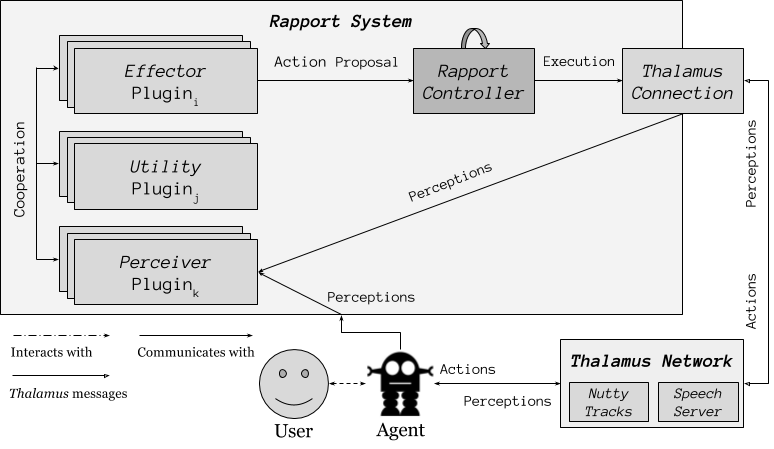
\includegraphics[width=0.9\textwidth]{images/RapportControllerArchitectureOverview.png}
	\caption{Schematic representation of the framework that implements the rapport model.}
	\label{fig:rapport:archicture}
\end{figure}

Following the same Figure~\ref{fig:rapport:archicture}, there are five types of connections:
\begin{itemize}
	\item \textbf{Perceptions}: perceptual information;
	\item \textbf{Actions}: decisive messages that trigger animations or utterances;
	\item \textbf{Action Proposal}: requests sent by \textit{Effector Plugins} that are managed by the \textit{Rapport Controller};
	\item \textbf{Execution}: set of actions triggered periodically by the \textit{Rapport Controller} - execution, interruptions or replacement according to the action proposals' stage;
	\item \textbf{Cooperation}: communication between plugins. For example, \textit{Effectors} use \textit{Perceivers} to read perceptual information and may use \textit{Utility} plugins to consult the interaction history.
\end{itemize}




